
% This LaTeX was auto-generated from MATLAB code.
% To make changes, update the MATLAB code and republish this document.

\documentclass{article}
\usepackage{graphicx}
\usepackage{color}

\sloppy
\definecolor{lightgray}{gray}{0.5}
\setlength{\parindent}{0pt}

\begin{document}

    
    \begin{verbatim}
function [ ] = Deber(  )
%Universidad de las Fuerzas Armadas
%Autor: Camilo Acosta
%Senales y Sistemas
%Deber de Convolucion

%Dado un sistema LTI discreto cuya entrada x[n] (senal en rojo) y respuesta impulsiva h[n] (senal verde) se
%muestran en las figuras. Obtenga la salida del sistema usando usando matlab.

%se limpia todas las variables del Workspace
clear all
%Se cierran todas las figuras
close all
%Para crear la primera senal discreta se crea un vector n que la delimite
n=-10:1:10;
%Dada la funcion Escalon definida por:
%......................................
%function [ h ] = escalon( n )
%h = n>=0;
%end
%......................................

%Usando la funcion escalon se crea una funcion "cuadrada" discreta, que va
%desde -10 a 10:
%x=(escalon(n+10)-escalon(n-11));
%A la anterior funcion se le multiplica por n para que x tome los mismos
%valores n, y se divide para dos para bajar la amplitud maxima de 10 a 5
%unidades.
x=(n/2).*(escalon(n+10)-escalon(n-11));

%Usando stem() se grafica de manera discreta x[n], de color rojo
stem(n,x,'r');
grid
xlabel('n')
ylabel('x[n]')
title('Senal x[n]')

%Para crear la primera senal discreta se crea un vector n2 que la delimite
n2=-4:1:4;

%Se crea un vector h1 que corresponde a los valores de h[n] ascendentes
%Se crea la funcion cuadrada a partir del escalon, que toma los valores desde 3 hasta cero
%Se lo multiplica por (n2+4), n2 para crear la pendiente ascendente y +4
%para desplazarlo verticalmente.
h1=(n2+4).*(escalon(n2+3)-escalon(n2-1));
%Se crea un vector h2 que corresponde a los valores de h[n] descendentes
%Se crea la funcion cuadrada a partir del escalon que toma los valores
%desde 1 hasta 3
%Se lo multiplica por (-n2+4), -n2 para crear la pendiente descendente y +4
%para desplazarlo verticalmente.
h2=(-n2+4).*(escalon(n2-1)-escalon(n2-4));
%Se suman h1 + h2 para creat el vector completo
h=h1+h2;

%Usando stem() se grafica de manera discreta h[n], de color verde
figure;
stem(n2,h,'g');
grid
xlabel('n')
ylabel('h[n]')
title('Senal h[n]')

%Se obtiene la convolucion usando conv()
y=conv(x,h);
figure
%n3=n+n2-1
%para saber la longitud de n3 se restan a ambos limites los limites
%inferiores de n=-10 y n2=-4
n3=-10-4:1:length(x)+length(h)-2-10-4;
%Usando stem() se grafica de manera discreta y[n], usando n3
stem(n3,y);
grid
xlabel('n')
ylabel('y[n]')
title('Senal y[n]')

end
\end{verbatim}

\includegraphics [width=4in]{Deber_01.eps}

\includegraphics [width=4in]{Deber_02.eps}

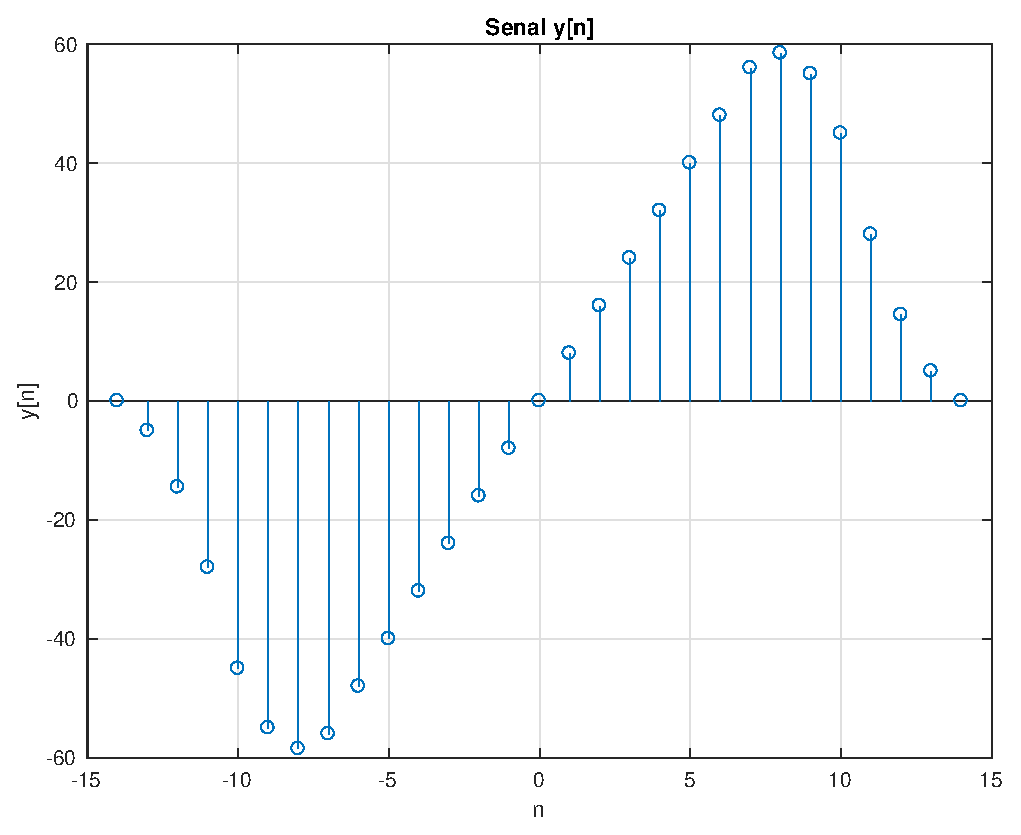
\includegraphics [width=4in]{Deber_03.eps}



\end{document}
    
